\documentclass[
  % all of the below options are optional and can be left out
  % course name (default: 2IL50 Data Structures)
  course = {{16-720B Computer Vision}},
  % quartile (default: 3)
  quartile = {{1}},
  % assignment number/name (default: 1)
  assignment = 4\ -\ Feature\ Descriptors\ \&\ Homographies\ \& \  RANSAC,
  % student name (default: Some One)
  name = {{Kangle Deng}},
  % student number, NOT S-number (default: 0123456)
  % studentnumber = {{0123456 ; 0314159}},
  % student email (default: s.one@student.tue.nl)
  email = {{kangled@andrew.cmu.edu}},
  % first exercise number (default: 1)
  firstexercise = 1
]{aga-homework}

\usepackage{url}
\usepackage{subfigure}

\begin{document}
\section{Keypoint Detector}

\noindent \textbf{Q1.2} See $keypointDetect.py$ for the implementation.

\noindent \textbf{Q1.3} Similarity of these 2 methods:

\begin{itemize}
    \item Both methods use Hessian-style partial derivatives.
\end{itemize}

Dissimilarity of these 2 methods:

\begin{itemize}
    \item Principle Curvature uses second derivatives while Harris uses first derivatives.
    \item Principle Curvature only calculates on one point while Harris calculate and sum on a patch around one point.
\end{itemize}

\noindent \textbf{Q1.4} See $keypointDetect.py$ for the implementation.

\noindent \textbf{Q1.5} Fig.\ref{fig:cv_hw4_q15} is the result.

\begin{figure}
    \centering
    \includegraphics{CV/fig/hw4/1_5.jpg}
    \caption{Q1.5: Result of DoG detector}
    \label{fig:cv_hw4_q15}
\end{figure}

\section{BRIEF Descriptor}

\noindent \textbf{Q2.1 Q2.2 Q2.3} See $BRIEF.py$ for the implementation.

% \noindent \textbf{Q2.2} See $BRIEF.py$ for the implementation.

% \noindent \textbf{Q2.3} See $BRIEF.py$ for the implementation.

\noindent \textbf{Q2.4} Fig. \ref{fig:cv_hw4_q241} and \ref{fig:cv_hw4_q242} are the results. In some cases (Fig. 2(b), 3(a), 3(b), 3(c) and 3(d)), there are a few mis-matches because there exist some objects similar to the object that we want to focus on. Also, rotated objects (Fig. 3(b) and 3(d)) are more difficult to match.

\begin{figure}
    \centering
    \subfigure[]{\includegraphics{CV/fig/hw4/1_4.pdf}}
    \subfigure[]{\includegraphics{CV/fig/hw4/1_41.pdf}}
    \caption{Q2.4 Result-A}
    \label{fig:cv_hw4_q241}
\end{figure}

\begin{figure}
    \centering
    \subfigure[]{\includegraphics[width = .48\textwidth]{CV/fig/hw4/1_4_book1.pdf}}
    \subfigure[]{\includegraphics[width = .48\textwidth]{CV/fig/hw4/1_4_book2.pdf}}
    \subfigure[]{\includegraphics[width = .48\textwidth]{CV/fig/hw4/1_4_book3.pdf}}
    \subfigure[]{\includegraphics[width = .48\textwidth]{CV/fig/hw4/1_4_book4.pdf}}
    \subfigure[]{\includegraphics[width = .48\textwidth]{CV/fig/hw4/1_4_book5.pdf}}
    \caption{Q2.4 Result-B}
    \label{fig:cv_hw4_q242}
\end{figure}

\noindent \textbf{Q2.5} Fig. \ref{fig:cv_hw4_q25} is the result. The number of matches are highest around 0 degrees and 360 degrees. This is because the rotation angle is so small that the view does not change much. However, BRIEF is not rotationally invariant, so the number of matches drop dramatically at other angles.  Also, the number of matches is relatively high at 90, 180, and 270. This is because our algorithm uses gradients along x-axis and y-axis to detect keypoints, so it is more sensitive to edges along x-axis and y-axis. When rotating 90, 180, and 270 degrees, those edges along x-axis and y-axis are still parallel to the axes. Therefore, the detected keypoints are more similar than those in other angles.

\begin{figure}
    \centering
    \includegraphics{CV/fig/hw4/q25.pdf}
    \caption{Q2.5: BRIEF and rotations}
    \label{fig:cv_hw4_q25}
\end{figure}

\section{Planar Homographies: Theory}
\noindent \textbf{Q3.1} 

\noindent \textbf{(a)} For each $\lambda \tilde{\mathbf{x}} = \mathbf{H} \tilde{\mathbf{u}}$ where $\tilde{\mathbf{x}} = [x, y, 1], H = [h1, h2, h3]^T$, we have:

\begin{equation*}
    \lambda \cdot \left(
    \begin{array}{c}
        x \\
        y \\
        1
    \end{array}
    \right) = \left(
    \begin{array}{c}
        h_1^T \\
        h_2^T \\
        h_3^T
    \end{array}
    \right) \cdot \tilde{\mathbf{u}}. 
\end{equation*}

So,

\begin{equation*}
    \begin{aligned}
        \lambda x & = h_1^T \tilde{\mathbf{u}}, \\
        \lambda y & = h_2^T \tilde{\mathbf{u}}, \\
        \lambda & = h_3^T \tilde{\mathbf{u}}.
    \end{aligned}
\end{equation*}

Eliminating $\lambda$, we have:
\begin{equation*}
    \begin{aligned}
        x & = h_1^T \tilde{\mathbf{u}} /  h_3^T \tilde{\mathbf{u}}, \\
        y & = h_2^T \tilde{\mathbf{u}} /  h_3^T \tilde{\mathbf{u}}.
    \end{aligned}
\end{equation*}

So,
\begin{equation*}
    \begin{aligned}
        h_1^T \tilde{\mathbf{u}} - x h_3^T \tilde{\mathbf{u}} & = 0 , \\
        h_2^T \tilde{\mathbf{u}} - y h_3^T \tilde{\mathbf{u}} & = 0.
    \end{aligned}
\end{equation*}
which is equivalent to:

\begin{equation*}
    \left(
    \begin{array}{ccc}
       \tilde{\mathbf{u}}^T  & 0 & -x\tilde{\mathbf{u}}^T \\
       0  & \tilde{\mathbf{u}}^T & -y\tilde{\mathbf{u}}^T
    \end{array}
    \right)_{2 \times 9} \cdot \left(
    \begin{array}{c}
         h_1  \\
         h_2 \\
         h_3
    \end{array}
    \right)_{9 \times 1} = 0.
\end{equation*}

This is for one correspondence. Stacking all of the $N$ correspondences, we have $2N$ independent linear equations:

\begin{equation*}
    \left(
    \begin{array}{ccc}
       \tilde{\mathbf{u}}^T_1  & 0 & -x_1\tilde{\mathbf{u}}^T_1 \\
       0  & \tilde{\mathbf{u}}^T_1 & -y_1\tilde{\mathbf{u}}^T_1 \\
       \cdots & \cdots & \cdots \\
       \tilde{\mathbf{u}}^T_n  & 0 & -x_n\tilde{\mathbf{u}}^T_n \\
       0  & \tilde{\mathbf{u}}^T_n & -y_n\tilde{\mathbf{u}}^T_n \\
    \end{array}
    \right)_{2N \times 9} \cdot \left(
    \begin{array}{c}
         h_1  \\
         h_2 \\
         h_3
    \end{array}
    \right)_{9 \times 1} = 0.
\end{equation*}

\noindent \textbf{(b)} There are 9 elements in $\mathbf{h}$.

\noindent \textbf{(c)} There are 8 degrees of freedom in $\mathbf{H}$, and each point correspondence gives information about 2 degrees of freedom. So at least 4 point pairs are required to solve this system.

\noindent \textbf{(d)} We can solve this system by
\begin{equation*}
    \hat{\mathbf{h}} = \arg\min \limits_{||\mathbf{h}||^2=1} ||\mathbf{A}\mathbf{h}||^2.
\end{equation*}
which is equivalent to:

\begin{equation*}
    \hat{\mathbf{h}} = \arg\min \frac{||\mathbf{A}\mathbf{h}||^2}{||\mathbf{h}||^2}.
\end{equation*}

From the Rayleigh quotient theorem, the solution is the column of $\mathbf{V}$ corresponding to smallest singular value, where $\mathbf{V}$ is obtained from SVD decomposition: $\mathbf{A} = \mathbf{U}\mathbf{\Sigma}\mathbf{V}^T$.

\noindent \textbf{Q3.2} Let Camera $A$ be the camera in the original position, Camera $B$ be the one to a rotation of $\theta$, and Camera $C$ be the one to a rotation of $2\theta$. Let $\mathbf{H}$ be the homography that maps from Camera $A$ to Camera $B$.

Since the rotation is about the camera centre and the camera intrinsic parameters have not changed, all of the 3 cameras have the same camera centre and intrinsic parameters. Therefore, the homography from Camera $A$ to $B$ is the same as the one from Camera $B$ to $C$.

So, given any point $\tilde{\mathbf{v}}$ in Camera $A$, $\mathbf{H}\tilde{\mathbf{v}}$ corresponds to the same point in Camera $B$. Then $\mathbf{H}\mathbf{H}\tilde{\mathbf{v}} = \mathbf{H}^2\tilde{\mathbf{v}}$ corresponds to the same point in Camera $C$. Therefore, $\mathbf{H}^2$ is the homography from Camera $A$ to $C$.

\noindent \textbf{Q3.3} Generally, the scene is not on a single plane in the world. Also, generally not only the camera orientations but also the positions change while changing the viewpoint. In those cases, the planar homography no longer holds.

\noindent \textbf{Q3.4} Any line in 3D can be represented by:

\begin{equation*}
    m^T\tilde{X} = 0,
\end{equation*}
where \tilde{X} is the homogeneous coordinates in 3D, and $m$ is the parameter of the line.

Given any point $\tilde{X}_0$ on this line, we project it onto 2D by $\tilde{x}_0 = P\tilde{X}_0$. We have:

\begin{equation*}
    (P^Tm)^T\tilde{x}_0 = m^T(P\tilde{x}_0) = m^T\tilde{X}_0 = 0.
\end{equation*}

So $\tilde{x}_0$ is on the line represented by $P^Tm$. Since the choice of $\tilde{X}_0$ is arbitrary, each point on the line $m$ in 3D corresponds to a point on the line $P^Tm$ in 2D.

\section{Planar Homographies: Implementation}

\noindent\textbf{Q4.1} See $planarH.py$ for the implementation.

\section{RANSAC}

\noindent\textbf{Q5.1} See $planarH.py$ for the implementation.

\section{Automated Homography Estimation and Warping}

\noindent \textbf{Q6.1} We should resize hp\_cover.jpg as pf\_scan\_scaled.jpg. Otherwise, the warped book-cover would not fill up the same space as the original book. Fig. \ref{fig:cv_hw4_q61} is the result. The $\mathbf{H}$ matrix is as follows:

\begin{verbatim}
[[ 7.87055381e-04 -7.45931978e-05  6.30737484e-01]
 [-1.09040558e-03  2.42131437e-03  7.75984372e-01]
 [-2.91721676e-06 -1.10702191e-07  3.28696625e-03]]
\end{verbatim}

\begin{figure}
    \centering
    \includegraphics[width=.6\textwidth]{CV/fig/hw4/6_1.jpg}
    \caption{Q6.1: Warped Result}
    \label{fig:cv_hw4_q61}
\end{figure}

\noindent \textbf{Q6.2} Tab. \ref{tab:cv_hw4_q62} is the result. More iterations our algorithm runs for, the better result $\mathbf{H}$ it would get. From Tab. \ref{tab:cv_hw4_q62}, we can see the performance gets better as max\_iters increase. On the other hand, both too small and too large tol values would lead to sub-optimal results. This is because too large tol values give not-so-accurate homography matrix while too small tol values would make the model too sensitive to noise.

A good selection for the number of random samples is the least number of samples required to fit a model. This ensures the least probability to include an outlier.

\begin{table}
  \begin{center}
    \begin{tabular}{lccc}
      \toprule
       & max\_iter = 500 & max\_iter = 5000 & max\_iter = 10000 \\
      \midrule
tol = 0.5 & \includegraphics[width=0.28\textwidth]{CV/fig/hw4/6_2_00.jpg} & \includegraphics[width=0.28\textwidth]{CV/fig/hw4/6_2_01.jpg}
& \includegraphics[width=0.28\textwidth]{CV/fig/hw4/6_2_02.jpg}\\
tol = 2 & \includegraphics[width=0.28\textwidth]{CV/fig/hw4/6_2_10.jpg} & \includegraphics[width=0.28\textwidth]{CV/fig/hw4/6_2_11.jpg}
& \includegraphics[width=0.28\textwidth]{CV/fig/hw4/6_2_12.jpg}\\
tol = 10 & \includegraphics[width=0.28\textwidth]{CV/fig/hw4/6_2_20.jpg} & \includegraphics[width=0.28\textwidth]{CV/fig/hw4/6_2_21.jpg}
& \includegraphics[width=0.28\textwidth]{CV/fig/hw4/6_2_22.jpg}\\
    \end{tabular}
  \end{center}
\caption{Q6.2: Ablation study of RANSAC parameters} 
  \label{tab:cv_hw4_q62}
\end{table}

\section{Stitching it together: Panoramas}

\noindent \textbf{Q7.1} Fig. \ref{fig:cv_hw4_q71} is the result. In the blending process, I use dynamic alpha blending for the center part (the region that 2 views intersect). That is to say, every pixel in the centre part of the final view is a weighted sum of the 2 views. Specifically, the closer the pixel is to the border of either view, the less weights we should put on this view. I calculate the distance from the border using a pre-defined function $cv2.distanceTransform$, which calculates the minimum distance from any 0 pixel for each pixel. Otherwise, if we use a fixed-weight alpha blending, the blending would not be seamless, which means we can clearly see the stitching border in the final view. However, using dynamic alpha blending gives a seamless final view.

\begin{figure}
    \centering
    \subfigure[Warped image]{\includegraphics[width=.9\textwidth]{CV/fig/hw4/7_1.jpg}}
    \subfigure[Stitching result]{
    \includegraphics[width=.9\textwidth]{CV/fig/hw4/q71.png}}
    \caption{Q7.1: Result of Image Stitching}
    \label{fig:cv_hw4_q71}
\end{figure}

\noindent \textbf{Q7.2} See $panoramas.py$ for the implementation.

\noindent \textbf{Q7.3} Fig. \ref{fig:cv_hw4_q73} is the result. The homography for Pittsburgh view is stored as $q73\_bestH\_1.npy$ while the other is stored as $q73\_bestH\_2.npy$. The algorithm gives a good panorama for Pittsburgh view while performs poorly at the keyboard image. I think the bad performance on the second case is because it's difficult to find correct matches from 2 views given so many confusing objects (different keys on the keyboard).

\begin{figure}
    \centering
    \subfigure{
    \includegraphics[width=.9\textwidth]{CV/fig/hw4/q721.png}}
    \subfigure{
    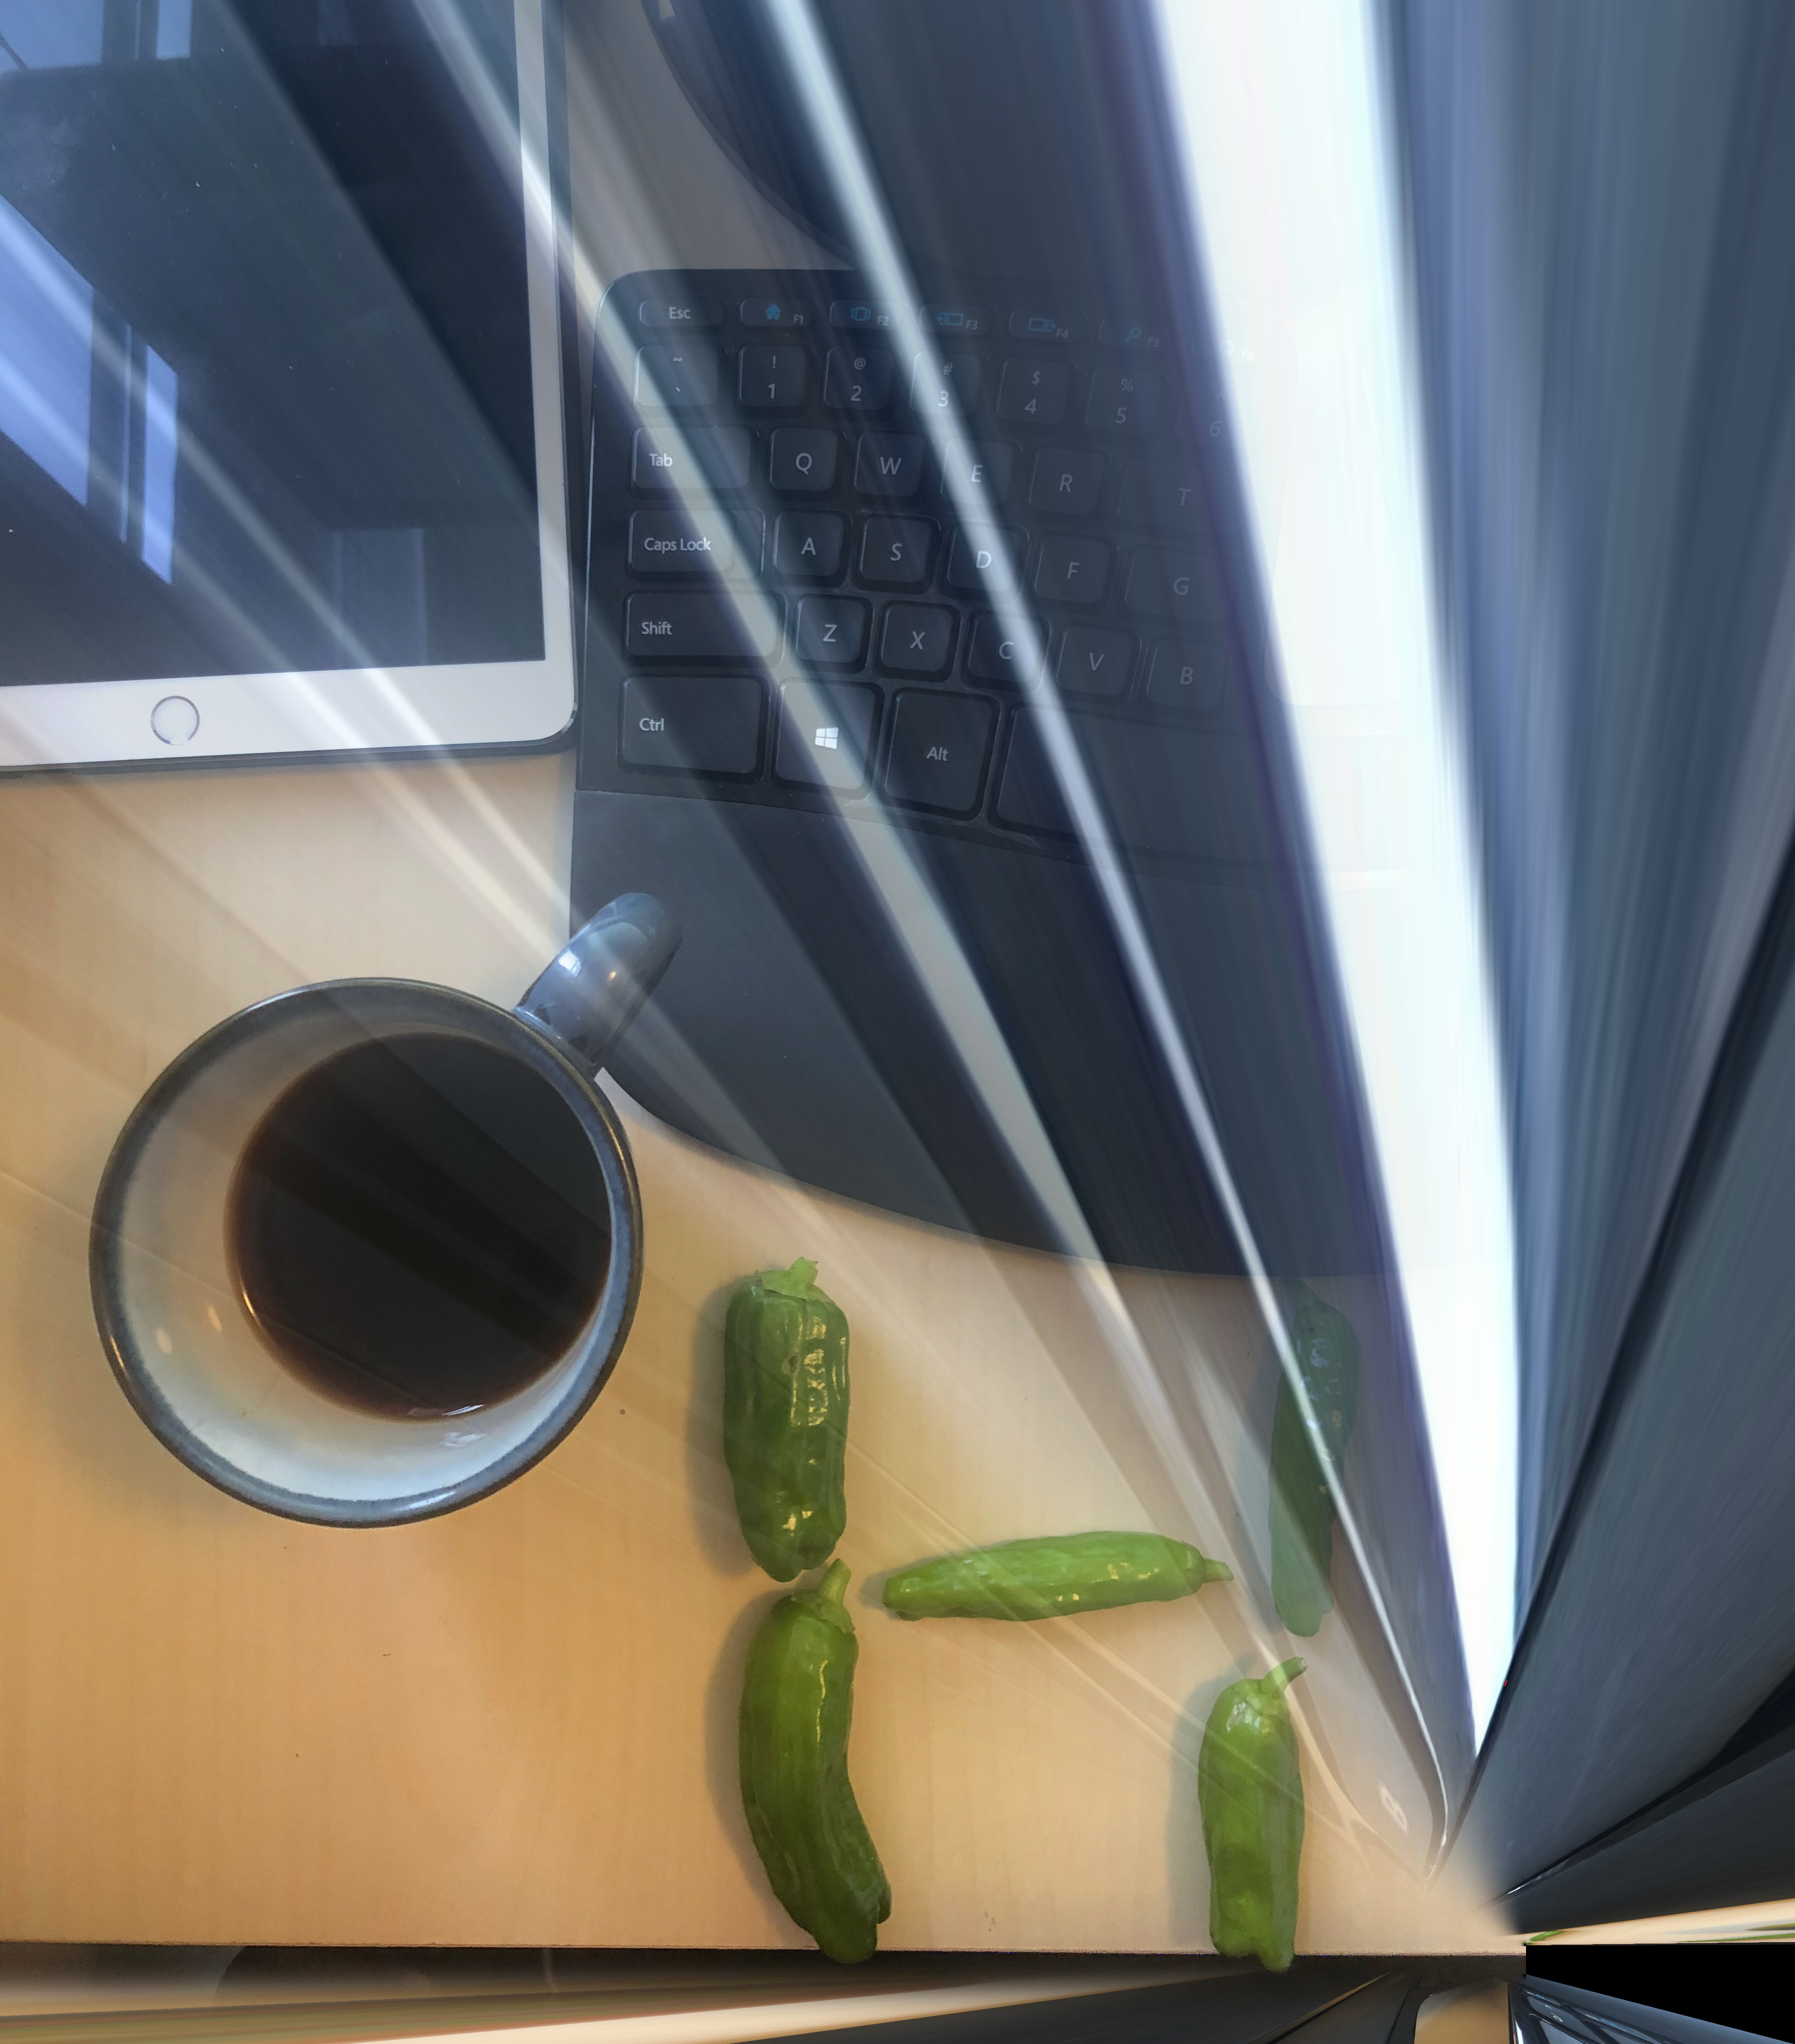
\includegraphics[width=.3\textwidth]{CV/fig/hw4/q722.png}}
    \caption{Q7.3: Result of No-clip Image Stitching}
    \label{fig:cv_hw4_q73}
\end{figure}

\section{Extra Credit}

\noindent \textbf{Q8.3} I use $skimage.feature.corner_orientations()$ to determine a principle direction for each keypoint. Then I rotate the patch that BRIEF is calculated on according to the principle direction. In this way, the indices of BRIEF descriptors keep same in spite of the rotation of images. Fig. \ref{fig:cv_hw4_q83_c} is an example. We can see that rotBRIEF provide more correct matches than BRIEF at a large rotation. Fig. \ref{fig:cv_hw4_q84} illustrates the number of matches at different rotation angles and scales. We can see that (compared to Fig. \ref{fig:cv_hw4_q25}), with rotBRIEF, there exist more matches when the object is rotated. However, rotBRIEF cannot find any matches at high scales such as 18, 19, and 20. See $ec\_1.py$ for the implementation.

\begin{figure}
    \centering
    \subfigure{
    \includegraphics[width=.48\textwidth]{CV/fig/hw4/q83_c1.png}}
    \subfigure{
    \includegraphics[width=.48\textwidth]{CV/fig/hw4/q83_c2.png}}
    \caption{Q8.3: Comparison between BRIEF (left) and rotBRIEF (right)}
    \label{fig:cv_hw4_q83_c}
\end{figure}

\begin{figure}
    \centering
    \subfigure{
    \includegraphics[width=.48\textwidth]{CV/fig/hw4/q83.pdf}}
    \subfigure{
    \includegraphics[width=.48\textwidth]{CV/fig/hw4/q83_scale.pdf}}
    \caption{Q8.3: Rotation and Scale for rotBRIEF}
    \label{fig:cv_hw4_q83}
\end{figure}

\noindent \textbf{Q8.4} I replace DoG with $\sigma^2-$scaled LoG, which is denoted as $\sigma^2\nabla^2G$. Fig. \ref{fig:cv_hw4_q84_example} is an example. We can see a lot of correct matches even though the image is scaled by 4 times. Fig. \ref{fig:cv_hw4_q84} illustrates the number of matches at different rotation angles and scales. We can see that, with LoG keypoint detector, the number of matches keeps consistent as the scale increases. On the other hand, LoG keypoint detector doesn't help with the cases about rotation. See $ec\_2.py$ for the implementation.

\begin{figure}
    \centering
    \includegraphics{CV/fig/hw4/q84_example.png}
    \caption{Q8.4: Example of matches between different scales (1 \times \quad v.s. \quad 4 \times)}
    \label{fig:cv_hw4_q84_example}
\end{figure}

\begin{figure}
    \centering
    \subfigure{
    \includegraphics[width=.48\textwidth]{CV/fig/hw4/q84_rotation.pdf}}
    \subfigure{
    \includegraphics[width=.48\textwidth]{CV/fig/hw4/q84_scale2.pdf}}
    \caption{Q8.4: Rotation and Scale for LoG detector}
    \label{fig:cv_hw4_q84}
\end{figure}

\end{document}
